\documentclass[11pt,a4paper]{article}
\usepackage[T1]{fontenc}
\usepackage[margin=2.3cm]{geometry}
\usepackage{amsmath,amssymb}
\usepackage{graphicx}
\usepackage[dvipsnames]{xcolor}
\usepackage{enumitem}
\usepackage[colorlinks=true,linkcolor=blue,urlcolor=blue]{hyperref}
\setlength{\parskip}{0.6em}
\setlength{\parindent}{0pt}
\begin{document}

\begin{center}{\LARGE\bfseries openproteinmd}\\[0.4em]{\large Fold a toy peptide on your own computer, in three sessions.}\\[0.2em]\small PAN IIT OSS explainer \textbullet{} secondary school to diploma / undergraduate (levels 3-5)\end{center}

\section*{Why this exists}
Molecular dynamics follows atoms by computing the force on each one and moving it a tiny step with Newton's law. This explainer builds that idea up from two atoms to a chain of beads, using only simple forces and a careful time-stepping rule, so you can build it yourself.

\section*{The end goal}
Fold a small peptide with molecular dynamics (general education). The end goal is a toy peptide that folds under molecular dynamics: a coarse-grained chain of hydrophobic and polar beads that collapses into a compact shape when it is cold enough. It is a teaching model, not a real protein, and nothing in it is medical or drug-design advice.

\section*{How the three sessions build up}
\begin{enumerate}[nosep]
\item \textbf{Session 1: Atoms as balls on springs: motion follows force} (Level 1, conceptual interactive model, 60 min).
\item \textbf{Session 2: Velocity Verlet: a time step you can trust} (Level 2, mathematical engineering model, 75 min).
\item \textbf{Session 3: A toy peptide folds: Langevin dynamics and validation} (Level 3, simulation and validation, 90 min).
\end{enumerate}

\section{Session 1: Atoms as balls on springs: motion follows force}

\subsection*{A. Real-world problem}
A protein is a long chain of atoms, far too small to watch. Scientists therefore simulate it: they write down the force on every atom and let Newton's law move the atoms a tiny step at a time. Before a whole chain, take the smallest possible case, two atoms. What pulls them together, what pushes them apart, and where do they settle? Important honesty note: everything in this repo is a toy model in made-up reduced units. It teaches how molecular dynamics works; it is not a real protein and not a tool for any medical or drug decision. General education only.

\subsection*{B. Concept and theory}
We measure length in sigma, energy in epsilon and mass in m, so all three equal 1; time then comes out in tau = sigma sqrt(m / epsilon). Two atoms at distance r interact through a potential energy V(r). The force is minus the slope: F = -dV/dr, positive when it pushes the atoms apart and negative when it pulls them together. A chemical bond is pictured as a spring, V = (1/2) k (r - r0)\textasciicircum{}2, with force F = -k (r - r0). Two atoms that are not bonded interact through the Lennard-Jones law, V = 4 [(1/r)\textasciicircum{}12 - (1/r)\textasciicircum{}6]: a steep repulsion at short range (the atoms cannot overlap) and a weak attraction at longer range. Its bottom is at r = 2\textasciicircum{}(1/6) sigma = 1.1225 sigma with depth -1 epsilon, and near the bottom it looks like a spring of constant 36 * 2\textasciicircum{}(2/3) = 57.15. A ball released away from the bottom is accelerated by the force and oscillates. Two equal atoms behave like one ball of reduced mass mu = m/2, so a spring pair has period 2 pi sqrt(mu / k). Our update rule is the simplest one: v\_new = v + (F / mu) dt, then r\_new = r + v\_new dt.

\begin{itemize}[nosep]
\item r: distance between the two atoms (sigma)
\item V: potential energy (epsilon)
\item F: force along the line joining the atoms (epsilon / sigma)
\item k: spring constant (epsilon / sigma\textasciicircum{}2)
\item r0: spring rest length (sigma)
\item mu: reduced mass of the pair (m/2) (m)
\item dt: time step (tau)
\end{itemize}

\begin{equation*}
F(r)=-\frac{dV}{dr}
\end{equation*}

\begin{equation*}
V_{\mathrm{spring}}=\tfrac12 k\,(r-r_0)^2,\qquad F_{\mathrm{spring}}=-k\,(r-r_0)
\end{equation*}

\begin{equation*}
V_{\mathrm{LJ}}=4\left[\left(\frac1r\right)^{12}-\left(\frac1r\right)^{6}\right],\qquad F_{\mathrm{LJ}}=\frac{24}{r}\left[2\left(\frac1r\right)^{12}-\left(\frac1r\right)^{6}\right]
\end{equation*}

\begin{equation*}
r_{\min}=2^{1/6}\sigma,\qquad V(r_{\min})=-\varepsilon,\qquad V''(r_{\min})=36\cdot 2^{2/3}\,\varepsilon/\sigma^2\approx 57.15
\end{equation*}

\begin{equation*}
T_{\mathrm{spring}}=2\pi\sqrt{\mu/k},\qquad \mu=m/2
\end{equation*}

\begin{center}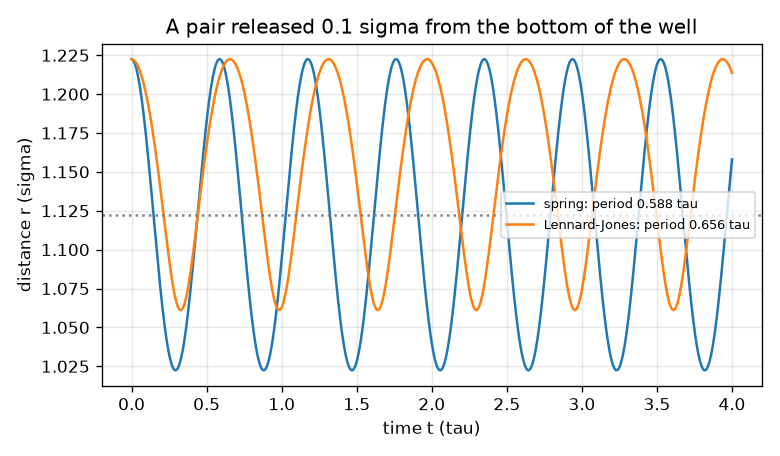
\includegraphics[width=0.85\linewidth]{figures/s01_pair_motion.png}\\\small A pair released 0.1 sigma from the bottom of the well: the spring period is 0.588 tau, the Lennard-Jones period is longer.\end{center}

\subsection*{E. Worked example}
Find the Lennard-Jones energy and force at r = 1.5 sigma. Is the pair pulled together or pushed apart?
\begin{enumerate}[nosep]
\item Compute (1/r)\textasciicircum{}6 = (1/1.5)\textasciicircum{}6 = 0.08779 and (1/r)\textasciicircum{}12 = 0.00771.
\item V = 4 (0.00771 - 0.08779) = 4 (-0.08008) = -0.3203 epsilon.
\item F = (24 / 1.5) [2 (0.00771) - 0.08779] = 16 (-0.07237) = -1.158 epsilon / sigma.
\item The force is negative, so the atoms are pulled together: r = 1.5 is outside the bottom of the well (1.1225), and the force points back towards it.
\item Check with the energy slope: V at 1.49 and 1.51 differ by about 0.0232 over 0.02 sigma, a slope of +1.16, and F = minus that slope = -1.16. The two ways agree.
\end{enumerate}
\textbf{Answer.} V = -0.3203 epsilon and F = -1.158 epsilon / sigma (attractive): the pair is pulled together.

\subsection*{F. Questions}
\begin{enumerate}[nosep]
\item \textbf{Conceptual.} A spring pair and a Lennard-Jones pair both oscillate about the same bottom. Why does the spring have a fixed period but the Lennard-Jones pair's period depends on how far you stretch it?
\item \textbf{Numerical.} A bond is modelled by a spring with k = 10 and r0 = 1. Find its energy and force at r = 1.3 (all in reduced units), and the Lennard-Jones energy and force at r = 2.
\item \textbf{Graph and simulation interpretation.} On the energy graph, where is the force zero, and what happens to a pair released at r = 1.6 sigma? Read it from the slope.
\item \textbf{Design and optimisation challenge.} Design: choose a spring constant so that a bond pair oscillates with a period of 0.5 tau, and say how large a time step you would then need to follow the motion with about 20 steps per period.
\end{enumerate}

\section{Session 2: Velocity Verlet: a time step you can trust}

\subsection*{A. Real-world problem}
To follow atoms we must take small time steps. If the stepping rule is poor, the computer atoms gain energy out of nothing and the simulation blows up; if the steps are too small, a run takes forever. How accurate must the rule be, how big can the step be, and how do we know the simulation is behaving? We answer on a case with an exact solution (one ball on a spring) and then on a small chain of beads. Toy model in reduced units, general education only.

\subsection*{B. Concept and theory}
Newton's law says a = F / m. We cannot solve it exactly for many atoms, so we advance in steps of length dt. Velocity Verlet does this in three moves: kick the velocity by half a step with the current force, drift the positions a full step, recompute the force at the new positions and kick the velocity by the second half step. It is time-reversible and it nearly conserves energy: the energy wobbles a little but does not drift. For a ball on a spring with angular frequency omega = sqrt(k / m) the largest relative energy error is about (omega dt)\textasciicircum{}2 / 4, and the method is stable only if omega dt \textless{} 2. The naive explicit Euler rule is different: it multiplies the energy by exactly (1 + (omega dt)\textasciicircum{}2) at every step, so the energy climbs without limit. A chain of N beads in d = 2 dimensions has potential energy U = sum of bond springs (1/2) K (l - R)\textasciicircum{}2 plus Lennard-Jones between non-neighbours. Temperature in molecular dynamics is defined from kinetic energy: T = 2 KE / (number of degrees of freedom), in units of epsilon / k\_B. When the total momentum is zero and conserved, d (N - 1) degrees of freedom count.

\begin{itemize}[nosep]
\item omega: angular frequency sqrt(k/m) of the fastest motion (1 / tau)
\item dt: time step (tau)
\item x, v, a: position, velocity, acceleration (sigma, sigma/tau, sigma/tau\textasciicircum{}2)
\item K: bond spring constant (100) (epsilon / sigma\textasciicircum{}2)
\item KE, U, E: kinetic, potential and total energy (epsilon)
\item N, d: number of beads and of dimensions (no unit)
\item T: kinetic temperature 2 KE / (d (N - 1)) (epsilon / k\_B)
\end{itemize}

\begin{equation*}
\mathbf v_{n+\frac12}=\mathbf v_n+\tfrac{\Delta t}{2}\,\mathbf a_n,\qquad \mathbf x_{n+1}=\mathbf x_n+\Delta t\,\mathbf v_{n+\frac12},\qquad \mathbf v_{n+1}=\mathbf v_{n+\frac12}+\tfrac{\Delta t}{2}\,\mathbf a_{n+1}
\end{equation*}

\begin{equation*}
\frac{\left|E-E_0\right|_{\max}}{E_0}\approx\frac{(\omega\,\Delta t)^2}{4},\qquad \text{stable only if }\ \omega\,\Delta t<2
\end{equation*}

\begin{equation*}
E_{n}^{\mathrm{Euler}}=E_0\,\big(1+\omega^2\Delta t^2\big)^{n}
\end{equation*}

\begin{equation*}
U=\sum_{\mathrm{bonds}}\tfrac12 K\,(l-R)^2+\sum_{|i-j|\ge 2}4\left[\left(\frac1{r_{ij}}\right)^{12}-\left(\frac1{r_{ij}}\right)^{6}\right]
\end{equation*}

\begin{equation*}
T=\frac{2\,\mathrm{KE}}{d\,(N-1)}
\end{equation*}

\begin{center}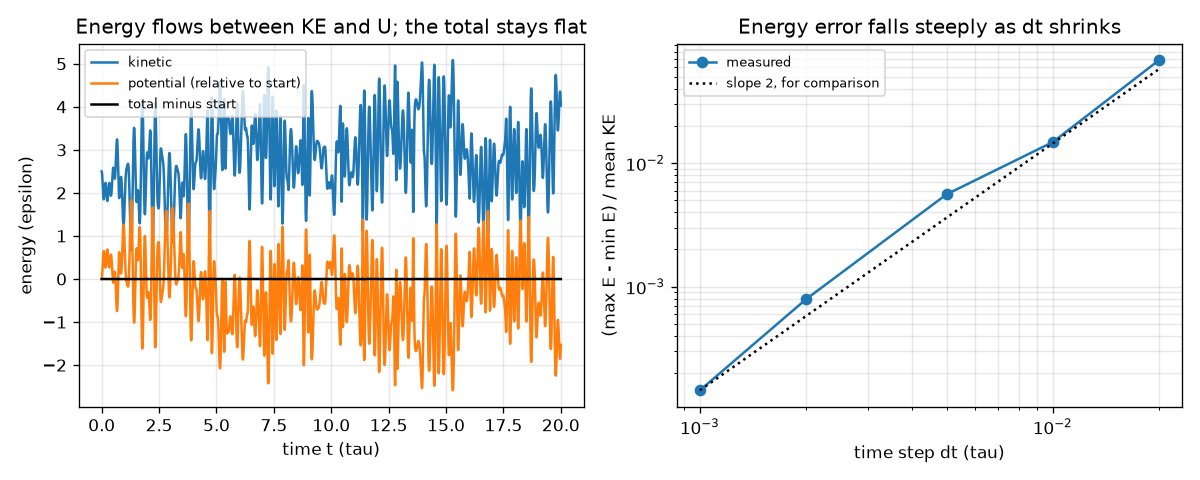
\includegraphics[width=0.85\linewidth]{figures/s02_chain_energy.png}\\\small A 6-bead chain at constant energy: energies trade places and the total stays flat (left); the energy error falls as the time step shrinks (right).\end{center}

\subsection*{E. Worked example}
A bond has omega = 10 per tau. What is the largest time step that keeps the Verlet energy error below 1 percent? What is the stability limit?
\begin{enumerate}[nosep]
\item Rule: error is about (omega dt)\textasciicircum{}2 / 4. We need (omega dt)\textasciicircum{}2 / 4 \textless{} 0.01.
\item So (omega dt)\textasciicircum{}2 \textless{} 0.04 and omega dt \textless{} 0.2, which gives dt \textless{} 0.2 / 10 = 0.02 tau.
\item Stability needs omega dt \textless{} 2, so dt \textless{} 2 / 10 = 0.2 tau, ten times larger than the accuracy limit.
\item Check by running it: the largest energy error over 20 periods is 0.0090 at dt = 0.019, 0.0100 at dt = 0.020 and 0.0110 at dt = 0.021; at dt = 0.21 (omega dt = 2.1) the energy blows up past a million times its start.
\end{enumerate}
\textbf{Answer.} dt must be below 0.02 tau for a 1 percent energy error; the method explodes beyond 0.2 tau.

\subsection*{F. Questions}
\begin{enumerate}[nosep]
\item \textbf{Conceptual.} Why does a poor integrator such as explicit Euler make the energy climb, while Verlet only makes it wobble?
\item \textbf{Numerical.} A 6-bead chain in 2D has zero total momentum and a total kinetic energy of 3.0 epsilon. What is its kinetic temperature? How many degrees of freedom did you use?
\item \textbf{Graph and simulation interpretation.} From the spring numbers (energy error 0.0025 at dt = 0.01 and 0.0625 at dt = 0.05, with omega = 10), what is the slope on a log-log plot and what does it tell you about halving the time step?
\item \textbf{Design and optimisation challenge.} Design: for a stiffer chain with K = 400 the fastest vibration has omega about 2 sqrt(K) = 40 per tau (an estimate from a harmonic chain). Choose the largest time step with energy error below 1 percent, and say what you give up.
\end{enumerate}

\section{Session 3: A toy peptide folds: Langevin dynamics and validation}

\subsection*{A. Real-world problem}
In water, the greasy (hydrophobic) parts of a protein hide together in the middle while the water-loving (polar) parts stay outside; this crowding is one of the main reasons that a chain collapses into a compact shape. How cold must a toy chain be to stay folded? We build the simplest cartoon of the idea, the HP model, run a real molecular dynamics simulation with a thermostat, validate it, and ask at which temperature the 12-bead sequence HPHPPHHPHPPH stays folded. Honest limits: this is a 12-bead toy in 2D with made-up reduced units. Real peptides have 3D backbones, side chains, water and charges, and fold on timescales millions of times longer than anything here. Nothing in this repo predicts a real protein and nothing here is medical or drug-design advice. General education only.

\subsection*{B. Concept and theory}
Every bead has mass 1 and is joined to its neighbours by a stiff spring (K = 100, rest length 1). Two H beads that are not neighbours attract through full Lennard-Jones (well depth 1 epsilon); every other non-neighbour pair only repels (the Lennard-Jones curve cut at its minimum and shifted up by 1, so it is zero beyond 2\textasciicircum{}(1/6) sigma). The pull between H beads stands in for the hydrophobic effect; the water itself is not simulated. To hold the temperature we add a heat bath with the Langevin equation: friction (gamma = 1) plus random kicks. The BAOAB scheme applies a half kick (B), a half drift (A), the friction-and-noise step (O) with c1 = exp(-gamma dt) and c2 = sqrt(T (1 - c1\textasciicircum{}2)), another half drift (A) and a half kick (B). The kicks balance the friction so that every degree of freedom carries on average T/2 of kinetic energy (equipartition); a Langevin bath does not conserve total momentum, so all d N degrees of freedom count, and T\_kin = 2 KE / (d N). The size of the chain is measured by the radius of gyration Rg, the root-mean-square distance of the beads from their centre. A straight chain of N beads with spacing 1 has Rg = sqrt((N\textasciicircum{}2 - 1) / 12). We call a chain folded when its mean Rg is below 1.8 sigma (a choice, not a law). The simulation is validated twice: the constant-energy run must conserve energy, and the thermostat must reproduce the set temperature.

\begin{itemize}[nosep]
\item T: set temperature of the heat bath (epsilon / k\_B)
\item gamma: friction rate of the bath (1) (1 / tau)
\item Rg: radius of gyration of the chain (sigma)
\item N: number of beads (12) (no unit)
\item dt: time step (0.01) (tau)
\item T\_kin: measured kinetic temperature 2 KE / (d N) (epsilon / k\_B)
\item contacts: number of non-neighbour H-H pairs closer than 1.5 sigma (no unit)
\end{itemize}

\begin{equation*}
U=\sum_{\mathrm{bonds}}\tfrac12 K\,(l-1)^2+\sum_{\substack{|i-j|\ge 2\\ \mathrm{both\ H}}}4\!\left[r^{-12}-r^{-6}\right]+\sum_{\substack{|i-j|\ge 2\\ \mathrm{otherwise}}}\left(4\!\left[r^{-12}-r^{-6}\right]+1\right)_{\,r<2^{1/6}}
\end{equation*}

\begin{equation*}
\mathbf v\leftarrow c_1\mathbf v+c_2\,\boldsymbol\xi,\qquad c_1=e^{-\gamma\Delta t},\quad c_2=\sqrt{T\left(1-c_1^2\right)},\quad \xi\sim\mathcal N(0,1)
\end{equation*}

\begin{equation*}
\langle \mathrm{KE}\rangle=\tfrac12\,d\,N\,T\quad\text{(equipartition)}
\end{equation*}

\begin{equation*}
R_g=\sqrt{\frac1N\sum_i\left|\mathbf r_i-\mathbf r_{\mathrm{cm}}\right|^2},\qquad R_g^{\mathrm{straight}}=\sqrt{\frac{N^2-1}{12}}
\end{equation*}

\begin{center}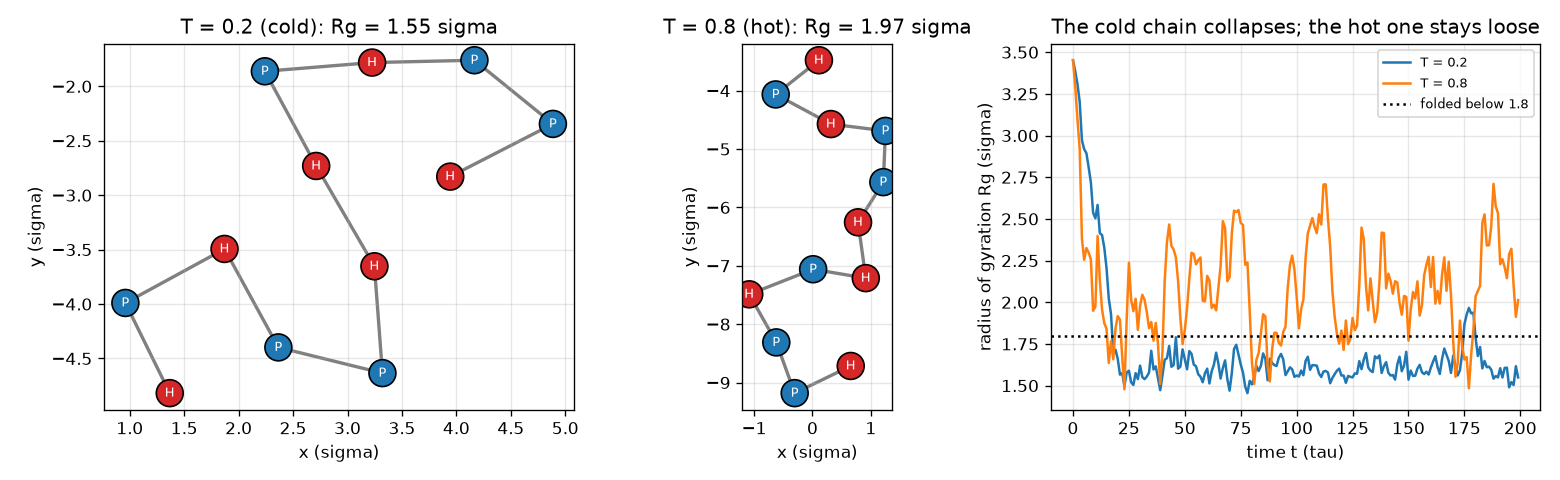
\includegraphics[width=0.85\linewidth]{figures/s03_collapse.png}\\\small A cold (T = 0.2) and a hot (T = 0.8) run of the 12-bead chain, and their radius of gyration against time.\end{center}

\subsection*{E. Worked example}
(a) What is the radius of gyration of the straight 12-bead chain? (b) At T = 0.5, what mean kinetic energy should the thermostat produce for 12 beads in 2D, and what does the simulation give?
\begin{enumerate}[nosep]
\item (a) Rg = sqrt((N\textasciicircum{}2 - 1) / 12) = sqrt(143 / 12) = sqrt(11.917) = 3.452 sigma. Code: radius\_of\_gyration(extended\_chain(12)) gives 3.452.
\item (b) Degrees of freedom: d N = 2 * 12 = 24 (the bath does not conserve momentum, so none is subtracted).
\item Equipartition: mean KE = (1/2) * 24 * 0.5 = 6.0 epsilon.
\item Run it: 20000 steps at T = 0.5 give a kinetic temperature of 0.508, so a mean KE of about 6.1 epsilon, within 2 percent of the prediction.
\item Hand check of Rg on a simpler shape: four beads at the corners of a unit square are each 0.707 from the centre, so Rg = 0.707 = sqrt(1/2).
\end{enumerate}
\textbf{Answer.} Rg of the straight chain is 3.452 sigma; at T = 0.5 the mean kinetic energy is 6.0 epsilon (simulation 6.1, T\_kin = 0.508).

\subsection*{F. Questions}
\begin{enumerate}[nosep]
\item \textbf{Conceptual.} The control chain PPPPPPPPPPPP never folds, even when cold, but HPHPPHHPHPPH does. What does that tell you about what causes the collapse in this model? And why does a correct equipartition temperature validate the thermostat but not the force field?
\item \textbf{Numerical.} A 12-bead chain in 2D is held at T = 0.6 by the Langevin bath. What mean kinetic energy do you expect? If a run reports a mean KE of 6.0, what is its kinetic temperature and what would you suspect?
\item \textbf{Graph and simulation interpretation.} In the lesson table of mean Rg against T (1.70 at T = 0.35, 1.87 at T = 0.40), at what temperature does the curve cross the folded line 1.8? Is there a sharp transition?
\item \textbf{Design and optimisation challenge.} Design: you want to simulate 100 tau of the chain at T = 0.3, at the lowest computer cost, with an energy spread (max minus min of E divided by mean KE) below 5 percent in a constant-energy check. Choose dt from the lesson measurements and count the steps.
\end{enumerate}

\section{Real-world mini-project}
\textbf{At which temperature does the 12-bead chain fold?.} Use \texttt{mean\_rg} and \texttt{RG\_FOLDED} from Session 3. The sequence is HPHPPHHPHPPH. For each temperature on the grid 0.30, 0.35, 0.40, 0.45, 0.50 (epsilon / k\_B) run 4 independent Langevin runs of 20000 steps with dt = 0.01 (seeds 1 to 4, \texttt{mean\_rg} does this for you) and call the chain folded when its mean radius of gyration is below 1.8 sigma. Report the folding temperature T* as the largest grid temperature that is still folded, and also an interpolated crossing between the two grid points that bracket 1.8. Run the control chain PPPPPPPPPPPP (no hydrophobic beads) on the same grid. This is a toy model: T* is a number for this cartoon only, not a property of any real peptide, and it depends on the 1.8 threshold you chose.

\section{The path ahead}
\begin{enumerate}[nosep]
\item \textbf{Session 4: A stiffer backbone.} Add the bending energy k (1 - cos phi), with phi the angle between consecutive bond vectors, to the 12-bead chain with k = 1.0.
\item \textbf{Session 5: Go 3D with a longer sequence.} A 3D chain of 20 beads, sequence PHPHHPPHPHHPPHPHHPHP, bending strength 0.5, cooled from T = 1.0 to 0.2 over 560 tau.
\item \textbf{Session 6: Error bars you can trust.} Extend the mini-project so that each temperature reports a mean Rg with a standard error.
\item \textbf{Session 7: Compare with the exact lattice model.} Enumerate every self-avoiding walk of 12 beads on a square lattice for HPHPPHHPHPPH and count H-H contacts.
\end{enumerate}

\section{Answers and hints}

\subsection*{Session 1}
\begin{enumerate}[nosep]
\item \textbf{Conceptual.} Hint: Compare the shape of the two energy curves away from the bottom. Solution: A spring has the same stiffness everywhere (a parabola), so its period 2 pi sqrt(mu/k) does not depend on the size of the swing. The Lennard-Jones well is not a parabola: it is steep on the inside and flattens out on the outside, so the farther you stretch the pair, the weaker the pull-back and the slower the motion. In the lesson a swing of 0.1 sigma gives a period of 0.656 tau and a swing of 0.5 sigma gives 1.609 tau. Only for very small swings does the Lennard-Jones pair behave like a spring.
\item \textbf{Numerical.} Hint: Use V = (1/2) k (r - r0)\textasciicircum{}2 and F = -k (r - r0); for Lennard-Jones compute (1/r)\textasciicircum{}6 first. Solution: Spring: V = 0.5 * 10 * 0.3\textasciicircum{}2 = 0.45 epsilon and F = -10 * 0.3 = -3.0 epsilon / sigma (pulls back). Lennard-Jones at r = 2: (1/2)\textasciicircum{}6 = 0.015625 and (1/2)\textasciicircum{}12 = 0.000244, so V = 4 (0.000244 - 0.015625) = -0.0615 epsilon and F = (24 / 2) (2 * 0.000244 - 0.015625) = 12 (-0.015137) = -0.1816 epsilon / sigma. Sanity check: at 2 sigma the attraction is already weak compared with the well depth of 1.
\item \textbf{Graph and simulation interpretation.} Hint: Force is minus the slope of V. Solution: The slope of V is zero at the bottom of the well, r = 1.123 sigma, so the force is zero there. At r = 1.6 the curve slopes upwards (V rises with r), so the force is negative: the atoms are pulled together, speed up towards the bottom, overshoot it where the force reverses sign, and oscillate. Without any friction they never settle (Session 3 adds the heat bath).
\item \textbf{Design and optimisation challenge.} Hint: Solve T = 2 pi sqrt(mu / k) for k with mu = 0.5. Then divide the period by 20. Solution: k = mu (2 pi / T)\textasciicircum{}2 = 0.5 * (2 pi / 0.5)\textasciicircum{}2 = 0.5 * 157.9 = 79.0, check: 2 pi sqrt(0.5 / 79) = 0.4999 tau. With 20 steps per period dt = 0.5 / 20 = 0.025 tau. Trade-off: a stiffer bond is a faster oscillation, so it forces a smaller time step and a longer run for the same simulated time. This is why Session 2 studies the time step carefully.
\end{enumerate}

\subsection*{Session 2}
\begin{enumerate}[nosep]
\item \textbf{Conceptual.} Hint: Think about what the update does to energy at each step, and about time reversibility. Solution: Explicit Euler multiplies the oscillator energy by exactly (1 + (omega dt)\textasciicircum{}2) each step, which is always greater than 1, so the energy grows exponentially, a systematic error that adds up. Velocity Verlet is time-reversible and symmetric: errors in one half step are undone by the other, and it exactly conserves a slightly modified energy, so the true energy only wobbles around its starting value without drifting. This is why molecular dynamics uses Verlet-type integrators.
\item \textbf{Numerical.} Hint: T = 2 KE / (d (N - 1)). Solution: Degrees of freedom: d (N - 1) = 2 * 5 = 10 (one set of 2 is used up by the fixed centre of mass). T = 2 * 3.0 / 10 = 0.6 epsilon / k\_B. Sanity check: a kinetic energy of 0.3 per degree of freedom is 0.5 T per degree, so T = 0.6 is consistent. Using N instead of N - 1 would give 0.5, an error of 20 percent for a chain this small.
\item \textbf{Graph and simulation interpretation.} Hint: Take the ratio of the errors and of the steps. Solution: The error ratio is 0.0625 / 0.0025 = 25 for a step ratio of 5, so error is proportional to dt\textasciicircum{}2 (5\textasciicircum{}2 = 25): slope 2. Halving the time step cuts the error by a factor of 4, but doubles the cost of a run. On the chain data the same trend is steeper or shallower in places because the chain has many frequencies; the dotted slope-2 line is only for comparison.
\item \textbf{Design and optimisation challenge.} Hint: Use omega dt \textless{} 0.2 and check that it is also below the stability limit 2 / omega. Solution: omega dt \textless{} 0.2 gives dt \textless{} 0.2 / 40 = 0.005 tau. The stability limit is 2 / 40 = 0.05 tau, so accuracy, not stability, sets the step. Compared with K = 100 (omega about 20, dt below 0.01) the cost of a run for the same simulated time doubles. The trade-off: stiffer bonds buy fidelity to a rigid bond length but cost computer time. Many real simulations freeze the fastest bonds to afford a larger step. This is an estimate: verify it with run\_nve.
\end{enumerate}

\subsection*{Session 3}
\begin{enumerate}[nosep]
\item \textbf{Conceptual.} Hint: Look at which pairs attract. Then think about what equipartition tests and what it cannot test. Solution: In this model only H-H pairs attract, so with no H beads there is nothing to gather: the all-P chain only has excluded volume and stays at Rg of about 2.2 sigma (2.17 to 2.28 on the grid of the mini-project). The collapse of the HP chain therefore comes from the H-H attraction. Equipartition checks the heat bath: the random kicks and friction are balanced so that the kinetic energy equals T/2 per degree of freedom. It says nothing about whether the potential energy is a good description of real molecules, so a thermostat can pass this test while the model is still a cartoon. The force code is validated separately (force equals minus the gradient of U, energy conserved in NVE).
\item \textbf{Numerical.} Hint: Use mean KE = (1/2) d N T and T\_kin = 2 KE / (d N) with d N = 24. Solution: Expected mean KE = 0.5 * 24 * 0.6 = 7.2 epsilon. For KE = 6.0, T\_kin = 2 * 6.0 / 24 = 0.5, which is 17 percent below the set 0.6. Far outside the 1 to 2 percent seen in the lesson, this would suggest a bug (for example the wrong number of degrees of freedom, an incorrect noise amplitude, or a run that is too short or has not yet reached equilibrium).
\item \textbf{Graph and simulation interpretation.} Hint: Linear interpolation between the two grid points. Solution: T = 0.35 + 0.05 * (1.8 - 1.70) / (1.87 - 1.70) = 0.35 + 0.05 * 0.59 = 0.38. The curve rises smoothly from 1.6 at T = 0.2 to 2.2 at T = 0.8 with no jump, so this is a gradual crossover and the 'folding temperature' depends on the 1.8 threshold we picked. Small chains (12 beads) have no sharp phase transition.
\item \textbf{Design and optimisation challenge.} Hint: The measured spreads over 20 tau are 5.0e-3 (dt 0.005), 1.9e-2 (0.01), 4.8e-2 (0.02), 0.18 (0.04) and 4.3 (0.08). Solution: dt = 0.02 is the largest tested step with a spread below 5 percent (4.8 percent), and dt = 0.04 (18 percent) is too big. The steps needed are 100 / 0.02 = 5000. Caveats: 4.8 percent is close to the limit, so dt = 0.01 (1.9 percent, 10000 steps) is the safer choice if the budget allows, and the spread was measured for the constant-energy run, not for the thermostatted one. Trade-off: halving dt doubles the cost; a dt of 0.15 makes the run blow up.
\end{enumerate}

\section{How to join}
Read \texttt{CONTRIBUTING.md} in the repository, then pick an issue labelled \texttt{good first issue}. Repository: \url{https://github.com/KrunalPanchal1995/openproteinmd}

\end{document}
